\documentclass[]{article}
\usepackage[linesnumbered,boxed]{algorithm2e}
\usepackage{amsmath}
\usepackage{graphicx}
%opening
\title{}
\author{}

\begin{document}
\title{Chapter 2 solution}
\maketitle

\begin{enumerate}
\item[2.1-1]

A = \{31, 41, 59, 26, 41, 58\} use insertion sort in ascending order

\noindent
After step 1:\\
	A = \{31, 41, 59, 26, 41, 58\}
	
After step 2:\\
	A = \{31, 41, 59, 26, 41, 58\}
	
After step 3:\\
	A = \{31, 41, 59, 26, 41, 58\}
	
After step 4:\\
	A = \{26, 31, 41, 59, 41, 58\}
	
After step 5:\\
	A = \{26, 31, 41, 41, 59, 58\}
	
After step 6:\\
	A = \{26, 31, 41, 41, 58, 59\}

\item[2.1-2] Rewrite insertion sort in descending order\\
Insertion-Sort(A)\\
1 for	j = 2 to A.length\\
2 \ \ \ \ key = A[j]\\
3 \ \ \ \ while i$>$0 and A[i]$<$key\\
4 \ \ \ \ \ \ \ \ A[i+1] = A[i]\\
5 \ \ \ \ \ \ \ \ i = i-1\\
6 \ \ \ \ A[i+1] = key\\

\item[2.1-3] Write pseudo-code for linear search problem\\
Linear-Search-Problem(A, v)\\
1 rt = NIL\\
2 for i = 1 to A.length\\
3 \ \ \ \ if A[i] == v\\
4 \ \ \ \ \ \ \ \ rt = i\\
5 \ \ \ \ \ \ \ \ break\\

\noindent
Proof:\\
Loop invariant: at iteration when i = k, v doesn't exist in A[1:k-1]\\
Initialization: i = 1, trivial case as there is nothing in A[1:0]\\
Maintenance: if v is in A[1:k-1] at A[j], then the loop will break when i=j\\
Termination: This is also obvious.

\item[2.1-4] Adding two n-bit binary integers A and B to (n+1) elements array C\\

Add-Binary-Integer(A, B)\\
1 int i=A.length\\
2 int j=B.length\\
3 allocate C as C[1:k] where k = max(i,j)+1\\
4 int m=max(i,j)+1\\
5 int carry = 0\\
6 while i$>$0 and j$ > $0\\
7 \ \ \ \ C[m] = A[i] xor B[j] xor carry\\
8 \ \ \ \ carry = (A[i] \& B[j]) $|$ (A[i] \& carry) $|$ (carry \& B[j])\\
9  m = m-1\\
10 i = i-1\\
11 j = j-1\\
12 while i$>$0 \\
13 \ \ \ \ C[m] = A[i] xor carry\\
14 \ \ \ \ carry = A[i] \& carry\\
15 \ \ \ \ i = i-1\\
16 \ \ \ \ m = m-1\\
17 while j$>$0 \\
18 \ \ \ \ C[m] = A[i] xor carry\\
19 \ \ \ \ carry = A[i] \& carry\\
20 \ \ \ \ j = j-1\\
21 \ \ \ \ m = m-1\\

\item[2.2-1] $$ n^3/1000 - 100n^2 -100n +3 = \Theta(n^3) $$

\item[2.2-2] Selection sort Loop invariant:\\
 before the i th iteration, the sub-array A[1:i-1] is sorted.\\
Within the i th iteration, the smallest element of the sub-array A[i:A.length] will be placed at A[i]\\

\noindent
Because after placing the first n-1 elements, the n th element is mutually at the right position.

\noindent
The best-case time complexity is $$ \Theta(n^2) $$
The worst-case time complexity is $$ \Theta(n^2) $$
There is no big difference in the best case and the worst case because it always takes (n-1)n/2 iterations, the difference is only about a constant number of operations within each iteration depending on whether we swap elements or not.

\item[2.2-3] The average number of elements needed to be checked is $$ \sum_{i=1}^{n}\frac{1}{n} * i = \frac{1+n}{2} $$
Worst case is n elements\\
Worst case time complexity: $$ \Theta(n) $$
Average case time complexity: $$ \Theta(n) $$

\item[2.2-4]
How to modify almost any algorithm to have a good best-case running time?\\
I am not sure, maybe storing the result for some special/frequent cases to achieve O(1) complexity in best case.

\item[2.3-1]Merge Sort on A = \{3, 41, 52, 26, 38, 57, 9, 49\}\\
This is very simple, just skip it.

\item[2.3-2] Rewrite Merge procedure so that it doesn't use sentinels, instead stopping once either array L or R has had all its elements copied back to A and then copying the reminder of the other array back into A.

//A: array\\
//L is A[p:q] R is A[q+1:r]\\
Merge(A, p, q, r)\\
1 let B[1:r-p+1] be a copy of A\\
2 i=p; j=q+1; k=1;\\
3 while i$<=$q and j$<=$r\\
4 \ \ \ \ if B[i]$<$B[j]\\
5 \ \ \ \ \ \ \ \ A[k] = B[i]\\
6 \ \ \ \ \ \ \ \ k=k+1; i=i+1;\\
7 \ \ \ \ else\\
8 \ \ \ \ \ \ \ \ A[k] = B[j]\\
9 \ \ \ \ \ \ \ \ k=k+1; j=j+1;\\
10 while i$<=$q\\
11 \ \ \ \ A[k]=B[i]\\
12 \ \ \ \ k=k+1; i=i+1;\\
13 while j$<=$r\\
14 \ \ \ \ A[k]=B[j]\\
15 \ \ \ \ k=k+1; j=j+1;\\

\item[2.3-3] Use mathematical induction to show that when n is an exact power of 2, the solution of the recurrence is $T(n) = n\lg(n)$

\[T(n) = \begin{cases}
2&\text{if n = 2},\\
2T(n/2) + n&\text{if $n=2^k$, for $k>1$}
\end{cases}\]

\noindent
For $n=2$, $T(2) = 2 \lg(2) = 2$

Suppose $T(n) = n\lg(n)\ \ \ \  \forall n=2^k<=m$

For $n=2^{k+1}$, $ T(2^{k+1}) = 2T(2^{k}) + 2^{k+1} = (k+1)2^{k+1} = 2^{k+1}\lg(2^{k+1}) $

By induction, it is proven that $T(n) = n\lg n$

\item[2.3-4] Recurrence relation of insertion sort

$$T(n) = T(n-1) + \Theta(n)$$

*$\Theta(n)$ depends on the position that A[n] is inserted.

\item[2.3-5] Binary-Search(A, v)

\begin{algorithm}[H]
\KwIn{A[1:n], v}
\KwOut{index}
$l=1; r=n$\\

\While{$ l<=r $}
{$i=(l+r)/2$\\
 \If{$A[i]=v$}
 {
 	return i
 }\ElseIf{$A[i]<v$}
 {
 	$l=i+1$
 }\Else{$r=i-1$}
}
\Return NIL
\end{algorithm}

\item[2.3-6] Yes we can. The dilemma is that we are not searching for a certain value, but the last element that is smaller than the given number or the first element that is larger than the given number.

The pseudo-code can be modified as follows

Insertion-Sort(A)\\
\begin{algorithm}[H]
\KwIn{A[1:n]}
\KwOut{A'[1:n] in sorted order}
\For{$ i=2; i<=n; i=i+1 $}
{
 $key=A[i]$\\
 $ l=1; r=i;$\\
 \While{$l<r$}
 {	
 	$m=(l+r)/2$\\
 	\If{$A[m]>key $}
 	{
 		$r=m-1$
 	}\Else{ $l=m-1$}
 }
 // now r is the last element that is smaller than key or
 the first element that is larger than key
 $k=-1$\\
 $t=-1$\\
 \If{$ A[l]<key $}
 {
 	$k=l$\\
 	$t=l+1$\\ 
 }\Else{
 	$k=l-1$\\
 	$t=l$\\
 }
 \For{$j=i-1; j>k; j=j-1$}
 {
 	$A[j+1]=A[j]$
 }
 $A[t]=key$
}
\Return A[]
\end{algorithm}

Skip the verification of runtime $\Theta (n\lg n)$

\item[2.3-7] Design a $\Theta (n\lg n)$-time algorithm that, given a set S of n integers and another integer x, determines whether or not there exist two elements in S whose sum is exactly x.\\

Since we have implemented SORT and BINARY-SEARCH, it is easy to this by sorting this set and then do a binary search for $x-A[i]$ on all n integers in S. Each search is $\Theta (\lg n)$ and the overall runtime will be $\Theta (n\lg n)$

\item[2-1] Mixture of insertion sort and merge sort\\
a. Sorting each sublist has runtime $\Theta(k^2)$. There are n/k sublists. Thus overall runtime is $\Theta(n/k*k^2) = \Theta(nk)$

b. We only need to draw the recursion tree.

\begin{figure}[!h]
\centering
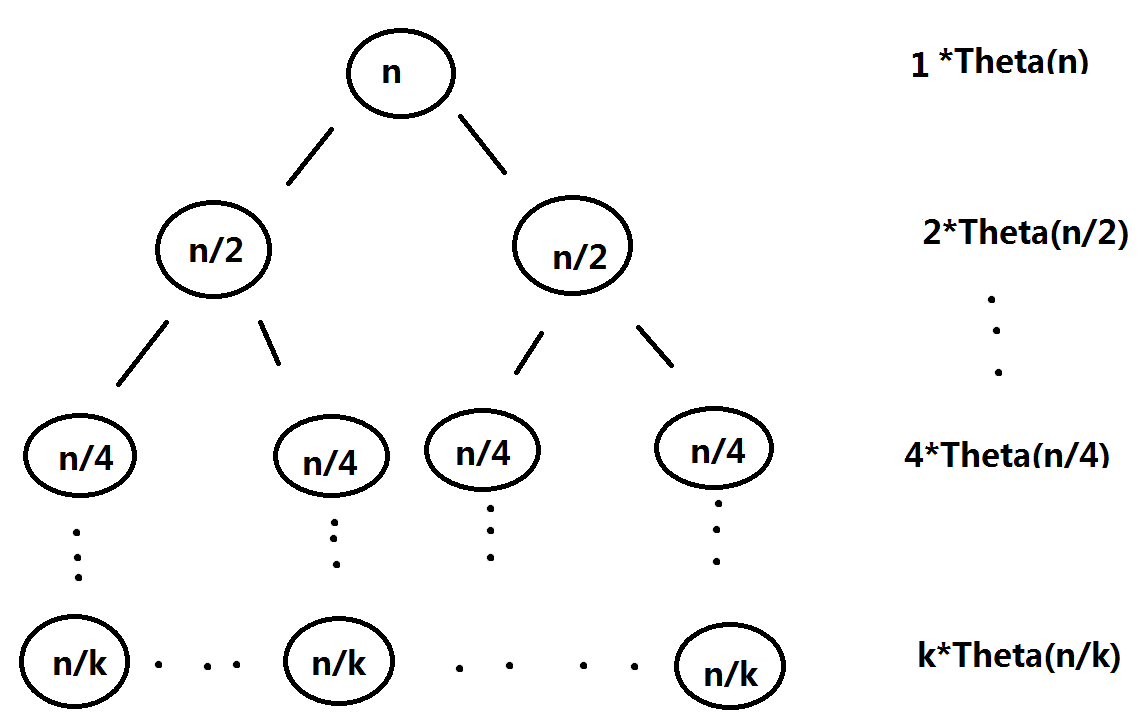
\includegraphics[width=0.7\linewidth]{./2-1RecursionTree}
\caption{Recursion tree for mixed sort}
\label{fig:2-1RecursionTree}
\end{figure}

The overall worst case runtime is merging time plus the worst case insertion sort time $$T(n) = \lg (n/k) * \Theta(n) + \Theta(nk) = \Theta(n\lg(n/k)) $$

c. Comparing $ \Theta(nk + n\lg(n/k)) $ with standard merge sort's runtime $\Theta(n\lg(n))$ is equivalent to comparing $ \Theta(k+\lg(n/k)) $ with $\Theta(\lg(n) )$

It is easy to guess that k can't exceed $\lg(n)$ asymptotically. Otherwise, the left hand side will exceed the right hand side asymptotically it it won't if vice versa.

d. Select k so that n/k is the largest number when insertion sort beats standard merge sort.

\item[2-2] Correctness of bubble sort\\

a. There still remains a subtle restriction that the new A' array must contain exactly all the original elements in A.

b. Loop invariant: at the entrance of each iteration, A[j:end] contains original elements of this range and A[j] is the smallest one among them. I'll skip the wordy justification with respect to initialization, maintain and termination.

c. Loop invariant: at the entrance of each iteration, A[1:i-1] is in sorted order. 

d. The worst case runtime is $ \Theta(n^2) $ as there will be (n-1)n/2 times comparisons when the array is in the exact descending order. Besides, there are much more swap operations than insertion sort, which cost more time copying memory.

\item[2-3] Correctness of Horner's rule\\
a. The runtime is $$ T(n)=\Theta(n) $$

b. \begin{algorithm}
	$y=0$
	\For{ i=0 to n }{
		$temp=a_i$\\
		\For{ j=1 to i}{
			$temp=temp*x$
		}
		$y=y+temp$
	}
	return y
\end{algorithm}

The runtime is $$T(n)=\Theta(n^2)$$

c. at i=n (entering the 1st loop), it sums from 0 to 1. This satisfies that the value of y is 0.

Suppose that when entering the loop i=m, $ y=\sum\limits_{k=0}^{n-(m+1)} a_{k+m+1}x^k $, after the code being executed, $ y=a_{m+1} + x*\sum\limits_{k=0}^{n-(m+1)} a_{k+m+1}x^k \\
= a_{m} + \sum\limits_{k=1}^{n-m} a_{k+m}x^k
= \sum\limits_{k=0}^{n-m} a_{k+m}x^k = Y(i=m-1) $

Thus the invariant is hold for all the iterations by induction.

d. By the loop invariant, at the end of the loop, the result would be $$ y=\sum\limits_{k=0}^{n} a_{k}x^k $$

which is directly equal to the result of the polynomial.

\item[2-4] Inversions\\
a. skip listing the inversions as they are trivial.

b. The array with the strict descending order has the most inversions. It has $(n-1 + n-2 + ... + 1) = \frac{(n-1)n}{2}$ inversions.

c. The number of shift operations will be the same number of the number of inversions. Thus they linearly proportional.

d. Merge-Sort(A, l, r)\\
\begin{algorithm}[H]
	\If{l=r}{
		return
	}
	m=(l+r)/2\\
	Merge-Sort(A, l, m)\\
	Merge-Sort(A, m+1, r)\\
	Merge(A, l, m, m+1, r)
\end{algorithm}

//assume that count is a global initialized to 0\\
Merge(A, l1, r1, l2, r2)\\
\begin{algorithm}[H]
	Copy A[l1:r2] to B[1:r2-l1+1]\\
	i=1; j=1+l2-l1; k=l1;\\
	\While{$ i<=r1 \ \text{and}\  j<=r2 $}{
		\If{$ B[i]<B[j] $}{
			A[k]=B[i]\\
			i=i+1\\
			k=k+1
		}\Else{
			A[k]=B[j]\\
			j=j+1\\
			k=k+1\\
			count = count+r1-i+1
		}
	}
	\While{$ i<=r1 $}{
		A[k]=B[i]\\
		i=i+1\\
		k=k+1
	}
	\While{$ j<=r2 $}{
		A[k]=B[j]\\
		j=j+1\\
		k=k+1\\
		count = count+r1-i+1	
	}
\end{algorithm}

After execution, count will be the number of inversions. The modification adds only constant number of operations of each subroutine, thus the runtime will still be $\Theta(n\lg(n))$


\end{enumerate}
\end{document}
